\documentclass[twoside]{book}

% Packages required by doxygen
\usepackage{fixltx2e}
\usepackage{calc}
\usepackage{doxygen}
\usepackage[export]{adjustbox} % also loads graphicx
\usepackage{graphicx}
\usepackage[utf8]{inputenc}
\usepackage{makeidx}
\usepackage{multicol}
\usepackage{multirow}
\PassOptionsToPackage{warn}{textcomp}
\usepackage{textcomp}
\usepackage[nointegrals]{wasysym}
\usepackage[table]{xcolor}

% Font selection
\usepackage[T1]{fontenc}
\usepackage[scaled=.90]{helvet}
\usepackage{courier}
\usepackage{amssymb}
\usepackage{sectsty}
\renewcommand{\familydefault}{\sfdefault}
\allsectionsfont{%
  \fontseries{bc}\selectfont%
  \color{darkgray}%
}
\renewcommand{\DoxyLabelFont}{%
  \fontseries{bc}\selectfont%
  \color{darkgray}%
}
\newcommand{\+}{\discretionary{\mbox{\scriptsize$\hookleftarrow$}}{}{}}

% Page & text layout
\usepackage{geometry}
\geometry{%
  a4paper,%
  top=2.5cm,%
  bottom=2.5cm,%
  left=2.5cm,%
  right=2.5cm%
}
\tolerance=750
\hfuzz=15pt
\hbadness=750
\setlength{\emergencystretch}{15pt}
\setlength{\parindent}{0cm}
\setlength{\parskip}{3ex plus 2ex minus 2ex}
\makeatletter
\renewcommand{\paragraph}{%
  \@startsection{paragraph}{4}{0ex}{-1.0ex}{1.0ex}{%
    \normalfont\normalsize\bfseries\SS@parafont%
  }%
}
\renewcommand{\subparagraph}{%
  \@startsection{subparagraph}{5}{0ex}{-1.0ex}{1.0ex}{%
    \normalfont\normalsize\bfseries\SS@subparafont%
  }%
}
\makeatother

% Headers & footers
\usepackage{fancyhdr}
\pagestyle{fancyplain}
\fancyhead[LE]{\fancyplain{}{\bfseries\thepage}}
\fancyhead[CE]{\fancyplain{}{}}
\fancyhead[RE]{\fancyplain{}{\bfseries\leftmark}}
\fancyhead[LO]{\fancyplain{}{\bfseries\rightmark}}
\fancyhead[CO]{\fancyplain{}{}}
\fancyhead[RO]{\fancyplain{}{\bfseries\thepage}}
\fancyfoot[LE]{\fancyplain{}{}}
\fancyfoot[CE]{\fancyplain{}{}}
\fancyfoot[RE]{\fancyplain{}{\bfseries\scriptsize Generated by Doxygen }}
\fancyfoot[LO]{\fancyplain{}{\bfseries\scriptsize Generated by Doxygen }}
\fancyfoot[CO]{\fancyplain{}{}}
\fancyfoot[RO]{\fancyplain{}{}}
\renewcommand{\footrulewidth}{0.4pt}
\renewcommand{\chaptermark}[1]{%
  \markboth{#1}{}%
}
\renewcommand{\sectionmark}[1]{%
  \markright{\thesection\ #1}%
}

% Indices & bibliography
\usepackage{natbib}
\usepackage[titles]{tocloft}
\setcounter{tocdepth}{3}
\setcounter{secnumdepth}{5}
\makeindex

% Hyperlinks (required, but should be loaded last)
\usepackage{ifpdf}
\ifpdf
  \usepackage[pdftex,pagebackref=true]{hyperref}
\else
  \usepackage[ps2pdf,pagebackref=true]{hyperref}
\fi
\hypersetup{%
  colorlinks=true,%
  linkcolor=blue,%
  citecolor=blue,%
  unicode%
}

% Custom commands
\newcommand{\clearemptydoublepage}{%
  \newpage{\pagestyle{empty}\cleardoublepage}%
}

\usepackage{caption}
\captionsetup{labelsep=space,justification=centering,font={bf},singlelinecheck=off,skip=4pt,position=top}

%===== C O N T E N T S =====

\begin{document}

% Titlepage & ToC
\hypersetup{pageanchor=false,
             bookmarksnumbered=true,
             pdfencoding=unicode
            }
\pagenumbering{roman}
\begin{titlepage}
\vspace*{7cm}
\begin{center}%
{\Large Motorcontrol wellplate reader }\\
\vspace*{1cm}
{\large Generated by Doxygen 1.8.11}\\
\end{center}
\end{titlepage}
\clearemptydoublepage
\tableofcontents
\clearemptydoublepage
\pagenumbering{arabic}
\hypersetup{pageanchor=true}

%--- Begin generated contents ---
\chapter{R\+E\+A\+D\+ME}
\label{md_README}
\hypertarget{md_README}{}
Start with \char`\"{}python3 main.\+py\char`\"{} 
\chapter{Hierarchical Index}
\section{Class Hierarchy}
This inheritance list is sorted roughly, but not completely, alphabetically\+:\begin{DoxyCompactList}
\item \contentsline{section}{main.\+depricated\+Functions}{\pageref{classmain_1_1depricated_functions}}{}
\item \contentsline{section}{serial\+\_\+printhat.\+Gcode\+Serial}{\pageref{classserial__printhat_1_1_gcode_serial}}{}
\item \contentsline{section}{stepper.\+Stepper\+Control}{\pageref{classstepper_1_1_stepper_control}}{}
\item Q\+Dialog\begin{DoxyCompactList}
\item \contentsline{section}{main.\+Main\+Window}{\pageref{classmain_1_1_main_window}}{}
\end{DoxyCompactList}
\item Q\+Object\begin{DoxyCompactList}
\item \contentsline{section}{stepper.\+signal\+Class}{\pageref{classstepper_1_1signal_class}}{}
\item \contentsline{section}{stepper.\+Stepper\+Wellpositioning}{\pageref{classstepper_1_1_stepper_wellpositioning}}{}
\end{DoxyCompactList}
\end{DoxyCompactList}

\chapter{Class Index}
\section{Class List}
Here are the classes, structs, unions and interfaces with brief descriptions\+:\begin{DoxyCompactList}
\item\contentsline{section}{\hyperlink{classmain_1_1depricated_functions}{main.\+depricated\+Functions} }{\pageref{classmain_1_1depricated_functions}}{}
\item\contentsline{section}{\hyperlink{classserial__printhat_1_1_gcode_serial}{serial\+\_\+printhat.\+Gcode\+Serial} }{\pageref{classserial__printhat_1_1_gcode_serial}}{}
\item\contentsline{section}{\hyperlink{classmain_1_1_main_window}{main.\+Main\+Window} }{\pageref{classmain_1_1_main_window}}{}
\item\contentsline{section}{\hyperlink{classstepper_1_1signal_class}{stepper.\+signal\+Class} }{\pageref{classstepper_1_1signal_class}}{}
\item\contentsline{section}{\hyperlink{classstepper_1_1_stepper_control}{stepper.\+Stepper\+Control} }{\pageref{classstepper_1_1_stepper_control}}{}
\item\contentsline{section}{\hyperlink{classstepper_1_1_stepper_wellpositioning}{stepper.\+Stepper\+Wellpositioning} }{\pageref{classstepper_1_1_stepper_wellpositioning}}{}
\end{DoxyCompactList}

\chapter{Class Documentation}
\hypertarget{classmain_1_1depricated_functions}{}\section{main.\+depricated\+Functions Class Reference}
\label{classmain_1_1depricated_functions}\index{main.\+depricated\+Functions@{main.\+depricated\+Functions}}
\subsection*{Public Member Functions}
\begin{DoxyCompactItemize}
\item 
def {\bfseries read\+Data} (self)\hypertarget{classmain_1_1depricated_functions_a2199d55c8b89dfb27c478823bf4ce536}{}\label{classmain_1_1depricated_functions_a2199d55c8b89dfb27c478823bf4ce536}

\end{DoxyCompactItemize}


The documentation for this class was generated from the following file\+:\begin{DoxyCompactItemize}
\item 
main.\+py\end{DoxyCompactItemize}

\hypertarget{classserial__printhat_1_1_gcode_serial}{}\section{serial\+\_\+printhat.\+Gcode\+Serial Class Reference}
\label{classserial__printhat_1_1_gcode_serial}\index{serial\+\_\+printhat.\+Gcode\+Serial@{serial\+\_\+printhat.\+Gcode\+Serial}}
\subsection*{Public Member Functions}
\begin{DoxyCompactItemize}
\item 
def {\bfseries \+\_\+\+\_\+init\+\_\+\+\_\+} (self)\hypertarget{classserial__printhat_1_1_gcode_serial_a286246832bdf1bc8dcf5ff82bdd74e6e}{}\label{classserial__printhat_1_1_gcode_serial_a286246832bdf1bc8dcf5ff82bdd74e6e}

\item 
def {\bfseries get\+Connection\+State} (self)\hypertarget{classserial__printhat_1_1_gcode_serial_a7402f098d751c69091a548d443abf72a}{}\label{classserial__printhat_1_1_gcode_serial_a7402f098d751c69091a548d443abf72a}

\item 
def {\bfseries set\+Connection\+State} (self, con\+State)\hypertarget{classserial__printhat_1_1_gcode_serial_a61995760948f024f83e28e0f0b0864ee}{}\label{classserial__printhat_1_1_gcode_serial_a61995760948f024f83e28e0f0b0864ee}

\item 
def {\bfseries connect} (self, port)\hypertarget{classserial__printhat_1_1_gcode_serial_a063eebd788e44d601f4d0e1836dab3a9}{}\label{classserial__printhat_1_1_gcode_serial_a063eebd788e44d601f4d0e1836dab3a9}

\item 
def {\bfseries execute\+Gcode} (self, gcode\+\_\+string)\hypertarget{classserial__printhat_1_1_gcode_serial_ac2da6000d16d939ee07933f4725cbec8}{}\label{classserial__printhat_1_1_gcode_serial_ac2da6000d16d939ee07933f4725cbec8}

\item 
def {\bfseries write\+GotoX} (self, pos)\hypertarget{classserial__printhat_1_1_gcode_serial_af5c18284e4e134be9d44b3b5b8be3058}{}\label{classserial__printhat_1_1_gcode_serial_af5c18284e4e134be9d44b3b5b8be3058}

\item 
def {\bfseries write\+GotoY} (self, pos)\hypertarget{classserial__printhat_1_1_gcode_serial_a7dd06397191df90fab761fc97b87623f}{}\label{classserial__printhat_1_1_gcode_serial_a7dd06397191df90fab761fc97b87623f}

\item 
def {\bfseries read\+Port} (self)\hypertarget{classserial__printhat_1_1_gcode_serial_ad891447bd77b7c72479275e963707aca}{}\label{classserial__printhat_1_1_gcode_serial_ad891447bd77b7c72479275e963707aca}

\item 
def {\bfseries disconnect} (self)\hypertarget{classserial__printhat_1_1_gcode_serial_a062d2321478b320d2e8fda8ec546d563}{}\label{classserial__printhat_1_1_gcode_serial_a062d2321478b320d2e8fda8ec546d563}

\end{DoxyCompactItemize}
\subsection*{Public Attributes}
\begin{DoxyCompactItemize}
\item 
{\bfseries connection\+State}\hypertarget{classserial__printhat_1_1_gcode_serial_a75cc30c7a97be0a19c799c9e3ebc8060}{}\label{classserial__printhat_1_1_gcode_serial_a75cc30c7a97be0a19c799c9e3ebc8060}

\item 
{\bfseries serial}\hypertarget{classserial__printhat_1_1_gcode_serial_a964d79ae702712d1c17196f8125843be}{}\label{classserial__printhat_1_1_gcode_serial_a964d79ae702712d1c17196f8125843be}

\end{DoxyCompactItemize}
\subsection*{Static Public Attributes}
\begin{DoxyCompactItemize}
\item 
int {\bfseries ins} = 0\hypertarget{classserial__printhat_1_1_gcode_serial_acfa7b28feeb6ce7c7f4d3c30bdc8e1b7}{}\label{classserial__printhat_1_1_gcode_serial_acfa7b28feeb6ce7c7f4d3c30bdc8e1b7}

\item 
bool {\bfseries connection\+State} = False\hypertarget{classserial__printhat_1_1_gcode_serial_a5307655ea0360555deb81d41e12e8039}{}\label{classserial__printhat_1_1_gcode_serial_a5307655ea0360555deb81d41e12e8039}

\end{DoxyCompactItemize}


The documentation for this class was generated from the following file\+:\begin{DoxyCompactItemize}
\item 
serial\+\_\+printhat.\+py\end{DoxyCompactItemize}

\hypertarget{classmain_1_1_main_window}{}\section{main.\+Main\+Window Class Reference}
\label{classmain_1_1_main_window}\index{main.\+Main\+Window@{main.\+Main\+Window}}


Inheritance diagram for main.\+Main\+Window\+:
\nopagebreak
\begin{figure}[H]
\begin{center}
\leavevmode
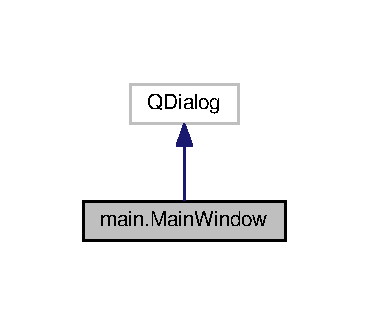
\includegraphics[width=177pt]{classmain_1_1_main_window__inherit__graph}
\end{center}
\end{figure}


Collaboration diagram for main.\+Main\+Window\+:
\nopagebreak
\begin{figure}[H]
\begin{center}
\leavevmode
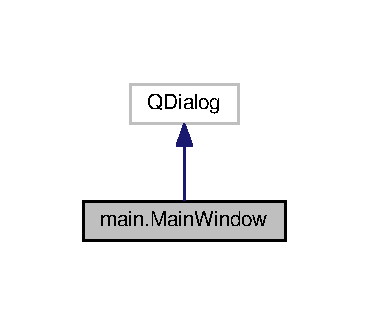
\includegraphics[width=177pt]{classmain_1_1_main_window__coll__graph}
\end{center}
\end{figure}
\subsection*{Public Member Functions}
\begin{DoxyCompactItemize}
\item 
def {\bfseries \+\_\+\+\_\+init\+\_\+\+\_\+} (self)\hypertarget{classmain_1_1_main_window_a549bdaddd0d7706c191be4046a97e6a4}{}\label{classmain_1_1_main_window_a549bdaddd0d7706c191be4046a97e6a4}

\item 
def {\bfseries create\+Batch\+Group\+Box} (self)\hypertarget{classmain_1_1_main_window_ae88202654b0d2dc5a8cd9a084feda42b}{}\label{classmain_1_1_main_window_ae88202654b0d2dc5a8cd9a084feda42b}

\item 
def {\bfseries create\+Manual\+Group\+Box} (self)\hypertarget{classmain_1_1_main_window_aa530c2ace70f4005bc537852144ffa89}{}\label{classmain_1_1_main_window_aa530c2ace70f4005bc537852144ffa89}

\item 
def {\bfseries create\+Log\+Window} (self)\hypertarget{classmain_1_1_main_window_a1d31fceddfe3542524643421c8a1914b}{}\label{classmain_1_1_main_window_a1d31fceddfe3542524643421c8a1914b}

\item 
def {\bfseries create\+Video\+Window} (self)\hypertarget{classmain_1_1_main_window_a0df93bd420fe59ac3f37081c435a680c}{}\label{classmain_1_1_main_window_a0df93bd420fe59ac3f37081c435a680c}

\item 
def {\bfseries Log\+Window\+Insert} (self, message)\hypertarget{classmain_1_1_main_window_afbf24d2ebf30574e064ec0dc9fe8b612}{}\label{classmain_1_1_main_window_afbf24d2ebf30574e064ec0dc9fe8b612}

\item 
def {\bfseries open\+Settings\+Ini\+File} (self)\hypertarget{classmain_1_1_main_window_a507bab9e21bd54d2f62a2b6aad118cda}{}\label{classmain_1_1_main_window_a507bab9e21bd54d2f62a2b6aad118cda}

\item 
def {\bfseries open\+Batch\+Ini\+File} (self)\hypertarget{classmain_1_1_main_window_ad1d8728bfd272170bac703bcc65d0fd5}{}\label{classmain_1_1_main_window_ad1d8728bfd272170bac703bcc65d0fd5}

\end{DoxyCompactItemize}
\subsection*{Public Attributes}
\begin{DoxyCompactItemize}
\item 
{\bfseries main\+Window\+Layout}\hypertarget{classmain_1_1_main_window_a5fa9093b94cd0244325eb2a8dae45fda}{}\label{classmain_1_1_main_window_a5fa9093b94cd0244325eb2a8dae45fda}

\item 
{\bfseries process\+Control\+Grid\+Layout}\hypertarget{classmain_1_1_main_window_a3b7f9ac4aa2fef39266892f620aefeeb}{}\label{classmain_1_1_main_window_a3b7f9ac4aa2fef39266892f620aefeeb}

\item 
{\bfseries batch\+Group\+Box}\hypertarget{classmain_1_1_main_window_aa3bd106e983803d3fcc0eed1732627c5}{}\label{classmain_1_1_main_window_aa3bd106e983803d3fcc0eed1732627c5}

\item 
{\bfseries b\+\_\+firmware\+\_\+restart}\hypertarget{classmain_1_1_main_window_ae0b5fb13ed24576de7a0a0acf9953204}{}\label{classmain_1_1_main_window_ae0b5fb13ed24576de7a0a0acf9953204}

\item 
{\bfseries b\+\_\+start\+\_\+batch}\hypertarget{classmain_1_1_main_window_a60a756fe9037d49c7d73fb4810ef784e}{}\label{classmain_1_1_main_window_a60a756fe9037d49c7d73fb4810ef784e}

\item 
{\bfseries b\+\_\+stop\+\_\+batch}\hypertarget{classmain_1_1_main_window_a4d7cf8763b813fca4c06d9a8e8c94976}{}\label{classmain_1_1_main_window_a4d7cf8763b813fca4c06d9a8e8c94976}

\item 
{\bfseries manual\+Control\+Grid\+Layout}\hypertarget{classmain_1_1_main_window_aaa83feeecab5fb158930435b571efb26}{}\label{classmain_1_1_main_window_aaa83feeecab5fb158930435b571efb26}

\item 
{\bfseries manual\+Group\+Box}\hypertarget{classmain_1_1_main_window_a87627928afa6f065ecf9657eb35c8389}{}\label{classmain_1_1_main_window_a87627928afa6f065ecf9657eb35c8389}

\item 
{\bfseries b\+\_\+home\+\_\+x}\hypertarget{classmain_1_1_main_window_a1a998f08fe166768a79cb079e11f2afb}{}\label{classmain_1_1_main_window_a1a998f08fe166768a79cb079e11f2afb}

\item 
{\bfseries b\+\_\+get\+\_\+pos}\hypertarget{classmain_1_1_main_window_a432b031cbe7470cee5357155c805588a}{}\label{classmain_1_1_main_window_a432b031cbe7470cee5357155c805588a}

\item 
{\bfseries b\+\_\+turn\+\_\+up}\hypertarget{classmain_1_1_main_window_a77164684a0f40fa0db807914b40ebf2b}{}\label{classmain_1_1_main_window_a77164684a0f40fa0db807914b40ebf2b}

\item 
{\bfseries b\+\_\+turn\+\_\+left}\hypertarget{classmain_1_1_main_window_a1a8d0a4527fe22beec110e98bb51afdf}{}\label{classmain_1_1_main_window_a1a8d0a4527fe22beec110e98bb51afdf}

\item 
{\bfseries b\+\_\+turn\+\_\+right}\hypertarget{classmain_1_1_main_window_a0f6440b38540725256a61f3528907fd7}{}\label{classmain_1_1_main_window_a0f6440b38540725256a61f3528907fd7}

\item 
{\bfseries b\+\_\+turn\+\_\+down}\hypertarget{classmain_1_1_main_window_a8ee34c2e103f8e6a0ac5591fcd36b97b}{}\label{classmain_1_1_main_window_a8ee34c2e103f8e6a0ac5591fcd36b97b}

\item 
{\bfseries x\+\_\+pos}\hypertarget{classmain_1_1_main_window_a4d4c2491cdb191c2a12e9cc282a13efc}{}\label{classmain_1_1_main_window_a4d4c2491cdb191c2a12e9cc282a13efc}

\item 
{\bfseries y\+\_\+pos}\hypertarget{classmain_1_1_main_window_ab4508f09fb201803ec924fb8fce79b2f}{}\label{classmain_1_1_main_window_ab4508f09fb201803ec924fb8fce79b2f}

\item 
{\bfseries b\+\_\+goto\+XY}\hypertarget{classmain_1_1_main_window_aafbc3bf9ef215a8e414cdf1817a8dfcc}{}\label{classmain_1_1_main_window_aafbc3bf9ef215a8e414cdf1817a8dfcc}

\item 
{\bfseries b\+\_\+emergency\+\_\+break}\hypertarget{classmain_1_1_main_window_a64fb3eaf720a7174276dd173376cac09}{}\label{classmain_1_1_main_window_a64fb3eaf720a7174276dd173376cac09}

\item 
{\bfseries log\+Grid\+Layout}\hypertarget{classmain_1_1_main_window_ae83014a31df8ed8a4c2865ec29a614d0}{}\label{classmain_1_1_main_window_ae83014a31df8ed8a4c2865ec29a614d0}

\item 
{\bfseries log\+Group\+Box}\hypertarget{classmain_1_1_main_window_a579eb24161cf122c768a94bb7aab4e9b}{}\label{classmain_1_1_main_window_a579eb24161cf122c768a94bb7aab4e9b}

\item 
{\bfseries log}\hypertarget{classmain_1_1_main_window_ab242000205fece5684ca25792ea01091}{}\label{classmain_1_1_main_window_ab242000205fece5684ca25792ea01091}

\item 
{\bfseries video\+Grid\+Layout}\hypertarget{classmain_1_1_main_window_ab3e8fcc5a6431ff01a4831d990d6cfa6}{}\label{classmain_1_1_main_window_ab3e8fcc5a6431ff01a4831d990d6cfa6}

\item 
{\bfseries video\+Group\+Box}\hypertarget{classmain_1_1_main_window_a91c103383e263695a268b582a501dc9f}{}\label{classmain_1_1_main_window_a91c103383e263695a268b582a501dc9f}

\item 
{\bfseries video\+Stream}\hypertarget{classmain_1_1_main_window_ad4da7c9249d2be9f7932580c811c1524}{}\label{classmain_1_1_main_window_ad4da7c9249d2be9f7932580c811c1524}

\end{DoxyCompactItemize}
\subsection*{Static Public Attributes}
\begin{DoxyCompactItemize}
\item 
{\bfseries message} = Signal(str)\hypertarget{classmain_1_1_main_window_a960ee91dc0975d9a75f899fac2b151d4}{}\label{classmain_1_1_main_window_a960ee91dc0975d9a75f899fac2b151d4}

\item 
{\bfseries Print\+H\+A\+T\+\_\+serial} = \hyperlink{classserial__printhat_1_1_gcode_serial}{serial\+\_\+printhat.\+Gcode\+Serial}()\hypertarget{classmain_1_1_main_window_af020947ae8a3a5f1bd978bb4f42934c0}{}\label{classmain_1_1_main_window_af020947ae8a3a5f1bd978bb4f42934c0}

\item 
{\bfseries settings} = None\hypertarget{classmain_1_1_main_window_a3c4bd8f7b4c501bee603a93207219660}{}\label{classmain_1_1_main_window_a3c4bd8f7b4c501bee603a93207219660}

\item 
{\bfseries settings\+\_\+batch} = None\hypertarget{classmain_1_1_main_window_a18f8a155a3fca9b3dada8a7d11c8674e}{}\label{classmain_1_1_main_window_a18f8a155a3fca9b3dada8a7d11c8674e}

\end{DoxyCompactItemize}


The documentation for this class was generated from the following file\+:\begin{DoxyCompactItemize}
\item 
main.\+py\end{DoxyCompactItemize}

\hypertarget{classstepper_1_1signal_class}{}\section{stepper.\+signal\+Class Class Reference}
\label{classstepper_1_1signal_class}\index{stepper.\+signal\+Class@{stepper.\+signal\+Class}}


Inheritance diagram for stepper.\+signal\+Class\+:
\nopagebreak
\begin{figure}[H]
\begin{center}
\leavevmode
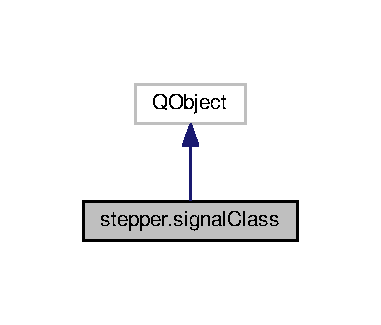
\includegraphics[width=183pt]{classstepper_1_1signal_class__inherit__graph}
\end{center}
\end{figure}


Collaboration diagram for stepper.\+signal\+Class\+:
\nopagebreak
\begin{figure}[H]
\begin{center}
\leavevmode
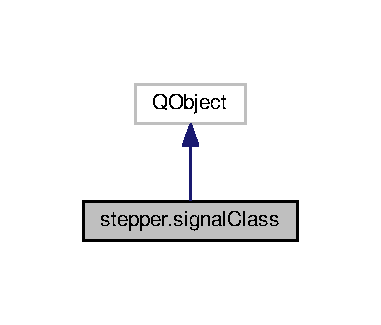
\includegraphics[width=183pt]{classstepper_1_1signal_class__coll__graph}
\end{center}
\end{figure}
\subsection*{Static Public Attributes}
\begin{DoxyCompactItemize}
\item 
{\bfseries sig} = Signal(str)\hypertarget{classstepper_1_1signal_class_a2bbd932799b1529a75912e5a1a45cf1a}{}\label{classstepper_1_1signal_class_a2bbd932799b1529a75912e5a1a45cf1a}

\end{DoxyCompactItemize}


The documentation for this class was generated from the following file\+:\begin{DoxyCompactItemize}
\item 
stepper.\+py\end{DoxyCompactItemize}

\hypertarget{classstepper_1_1_stepper_control}{}\section{stepper.\+Stepper\+Control Class Reference}
\label{classstepper_1_1_stepper_control}\index{stepper.\+Stepper\+Control@{stepper.\+Stepper\+Control}}
\subsection*{Public Member Functions}
\begin{DoxyCompactItemize}
\item 
def {\bfseries \+\_\+\+\_\+init\+\_\+\+\_\+} (self)\hypertarget{classstepper_1_1_stepper_control_a9da54e50265bfda0d3f8545e3f2e7bfc}{}\label{classstepper_1_1_stepper_control_a9da54e50265bfda0d3f8545e3f2e7bfc}

\item 
def {\bfseries msg} (self, message)\hypertarget{classstepper_1_1_stepper_control_aa8dc51da2ee0fb7516b6387af022c54b}{}\label{classstepper_1_1_stepper_control_aa8dc51da2ee0fb7516b6387af022c54b}

\item 
def {\bfseries get\+Position} (self)\hypertarget{classstepper_1_1_stepper_control_a167fb65d8b1fcfe526814be53ebfb90c}{}\label{classstepper_1_1_stepper_control_a167fb65d8b1fcfe526814be53ebfb90c}

\item 
def {\bfseries set\+Position} (self, pos)\hypertarget{classstepper_1_1_stepper_control_a7e09779dfbb8f133108585172825ad7e}{}\label{classstepper_1_1_stepper_control_a7e09779dfbb8f133108585172825ad7e}

\item 
def {\bfseries homeX} (self)\hypertarget{classstepper_1_1_stepper_control_ae85703b3df24016a6764e44b62c5d558}{}\label{classstepper_1_1_stepper_control_ae85703b3df24016a6764e44b62c5d558}

\item 
def {\bfseries homeY} (self)\hypertarget{classstepper_1_1_stepper_control_a8be471a3eff314d54f89c1dfe5cd5762}{}\label{classstepper_1_1_stepper_control_a8be471a3eff314d54f89c1dfe5cd5762}

\item 
def {\bfseries gotoX} (self, pos)\hypertarget{classstepper_1_1_stepper_control_ab5f6f529f7e1ad7eaec1ccd71e126b4f}{}\label{classstepper_1_1_stepper_control_ab5f6f529f7e1ad7eaec1ccd71e126b4f}

\item 
def {\bfseries gotoY} (self, pos)\hypertarget{classstepper_1_1_stepper_control_a32fc69a38aca1503e8f8f0f35ccf4228}{}\label{classstepper_1_1_stepper_control_a32fc69a38aca1503e8f8f0f35ccf4228}

\item 
def {\bfseries turn\+Up} (self)\hypertarget{classstepper_1_1_stepper_control_a5f0cf3f69d31cdfc4d3667a64ad341d0}{}\label{classstepper_1_1_stepper_control_a5f0cf3f69d31cdfc4d3667a64ad341d0}

\item 
def {\bfseries turn\+Left} (self)\hypertarget{classstepper_1_1_stepper_control_a4b7c3ae549af80504fd468f217d206cf}{}\label{classstepper_1_1_stepper_control_a4b7c3ae549af80504fd468f217d206cf}

\item 
def {\bfseries turn\+Right} (self)\hypertarget{classstepper_1_1_stepper_control_a5af585807c0a542f56ab03542ac681a4}{}\label{classstepper_1_1_stepper_control_a5af585807c0a542f56ab03542ac681a4}

\item 
def {\bfseries turn\+Down} (self)\hypertarget{classstepper_1_1_stepper_control_a48e1648f38637aed141f495747564bdd}{}\label{classstepper_1_1_stepper_control_a48e1648f38637aed141f495747564bdd}

\end{DoxyCompactItemize}
\subsection*{Public Attributes}
\begin{DoxyCompactItemize}
\item 
{\bfseries position}\hypertarget{classstepper_1_1_stepper_control_a983bf6e742834359344ff84758112cab}{}\label{classstepper_1_1_stepper_control_a983bf6e742834359344ff84758112cab}

\end{DoxyCompactItemize}
\subsection*{Static Public Attributes}
\begin{DoxyCompactItemize}
\item 
{\bfseries message} = Signal(str)\hypertarget{classstepper_1_1_stepper_control_af58d6597631c652cea9f9c9b4486ca3f}{}\label{classstepper_1_1_stepper_control_af58d6597631c652cea9f9c9b4486ca3f}

\end{DoxyCompactItemize}


The documentation for this class was generated from the following file\+:\begin{DoxyCompactItemize}
\item 
stepper.\+py\end{DoxyCompactItemize}

\hypertarget{classstepper_1_1_stepper_wellpositioning}{}\section{stepper.\+Stepper\+Wellpositioning Class Reference}
\label{classstepper_1_1_stepper_wellpositioning}\index{stepper.\+Stepper\+Wellpositioning@{stepper.\+Stepper\+Wellpositioning}}


Inheritance diagram for stepper.\+Stepper\+Wellpositioning\+:
\nopagebreak
\begin{figure}[H]
\begin{center}
\leavevmode
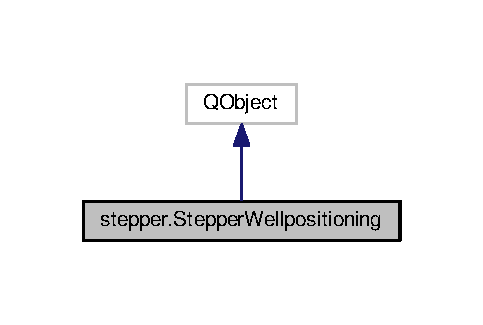
\includegraphics[width=232pt]{classstepper_1_1_stepper_wellpositioning__inherit__graph}
\end{center}
\end{figure}


Collaboration diagram for stepper.\+Stepper\+Wellpositioning\+:
\nopagebreak
\begin{figure}[H]
\begin{center}
\leavevmode
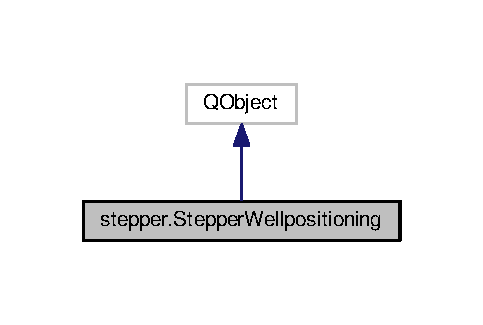
\includegraphics[width=232pt]{classstepper_1_1_stepper_wellpositioning__coll__graph}
\end{center}
\end{figure}
\subsection*{Public Member Functions}
\begin{DoxyCompactItemize}
\item 
def {\bfseries \+\_\+\+\_\+init\+\_\+\+\_\+} (self, stepperX, stepperY, gcode\+Serial)\hypertarget{classstepper_1_1_stepper_wellpositioning_a39fd3eeef150ae1fdaa5a63c5cac1904}{}\label{classstepper_1_1_stepper_wellpositioning_a39fd3eeef150ae1fdaa5a63c5cac1904}

\item 
def {\bfseries msg} (self, message)\hypertarget{classstepper_1_1_stepper_wellpositioning_a970090d87894de2fe922df0bf248cfae}{}\label{classstepper_1_1_stepper_wellpositioning_a970090d87894de2fe922df0bf248cfae}

\item 
def {\bfseries reset\+\_\+current\+\_\+well} (self)\hypertarget{classstepper_1_1_stepper_wellpositioning_a80852795d8751db5b8d351d0d94c3b38}{}\label{classstepper_1_1_stepper_wellpositioning_a80852795d8751db5b8d351d0d94c3b38}

\item 
def {\bfseries set\+\_\+current\+\_\+well} (self, x, y)\hypertarget{classstepper_1_1_stepper_wellpositioning_aa354e3491d1ec6f2c1ed1053a08f7191}{}\label{classstepper_1_1_stepper_wellpositioning_aa354e3491d1ec6f2c1ed1053a08f7191}

\item 
def {\bfseries get\+\_\+current\+\_\+well} (self)\hypertarget{classstepper_1_1_stepper_wellpositioning_a99c1c7961cbe3b6b22c74d4883726eba}{}\label{classstepper_1_1_stepper_wellpositioning_a99c1c7961cbe3b6b22c74d4883726eba}

\item 
def {\bfseries wait\+\_\+ms} (self, milliseconds)\hypertarget{classstepper_1_1_stepper_wellpositioning_ac89fd6526aeb8b4ccd17924252ee9250}{}\label{classstepper_1_1_stepper_wellpositioning_ac89fd6526aeb8b4ccd17924252ee9250}

\item 
def {\bfseries goto\+\_\+wel} (self, x\+\_\+pos, y\+\_\+pos)\hypertarget{classstepper_1_1_stepper_wellpositioning_aacfe7748cea3d2531e6cd8f73d33f84b}{}\label{classstepper_1_1_stepper_wellpositioning_aacfe7748cea3d2531e6cd8f73d33f84b}

\item 
def {\bfseries firmware\+Restart} (self)\hypertarget{classstepper_1_1_stepper_wellpositioning_adcd22bc691835b5398a56318f5b8a5ac}{}\label{classstepper_1_1_stepper_wellpositioning_adcd22bc691835b5398a56318f5b8a5ac}

\item 
def {\bfseries homeX} (self)\hypertarget{classstepper_1_1_stepper_wellpositioning_ab0dc8a7bd73180858832ddb1888227f6}{}\label{classstepper_1_1_stepper_wellpositioning_ab0dc8a7bd73180858832ddb1888227f6}

\item 
def {\bfseries get\+Position} (self)\hypertarget{classstepper_1_1_stepper_wellpositioning_a851a52db0708513a63030816804ab594}{}\label{classstepper_1_1_stepper_wellpositioning_a851a52db0708513a63030816804ab594}

\item 
def {\bfseries turn\+Up} (self)\hypertarget{classstepper_1_1_stepper_wellpositioning_a0bb04faad0a2bc6bd2bd33e42fda7ac2}{}\label{classstepper_1_1_stepper_wellpositioning_a0bb04faad0a2bc6bd2bd33e42fda7ac2}

\item 
def {\bfseries turn\+Left} (self)\hypertarget{classstepper_1_1_stepper_wellpositioning_a236a9d0dd741c77ef44343f58ebe2af7}{}\label{classstepper_1_1_stepper_wellpositioning_a236a9d0dd741c77ef44343f58ebe2af7}

\item 
def {\bfseries turn\+Right} (self)\hypertarget{classstepper_1_1_stepper_wellpositioning_a39800e8b3d9564efa09a8694f7e1ab72}{}\label{classstepper_1_1_stepper_wellpositioning_a39800e8b3d9564efa09a8694f7e1ab72}

\item 
def {\bfseries turn\+Down} (self)\hypertarget{classstepper_1_1_stepper_wellpositioning_a9d67b60ed3129543dfd72f0f3521155d}{}\label{classstepper_1_1_stepper_wellpositioning_a9d67b60ed3129543dfd72f0f3521155d}

\item 
def {\bfseries goto\+XY} (self, posX, posY)\hypertarget{classstepper_1_1_stepper_wellpositioning_a1253c08ba4da2318fb0cfdbcca391f36}{}\label{classstepper_1_1_stepper_wellpositioning_a1253c08ba4da2318fb0cfdbcca391f36}

\item 
def {\bfseries emergency\+Break} (self)\hypertarget{classstepper_1_1_stepper_wellpositioning_a7c2f4dab6111e79e3bed11c24fe2b6cc}{}\label{classstepper_1_1_stepper_wellpositioning_a7c2f4dab6111e79e3bed11c24fe2b6cc}

\end{DoxyCompactItemize}
\subsection*{Static Public Attributes}
\begin{DoxyCompactItemize}
\item 
{\bfseries message} = \hyperlink{classstepper_1_1signal_class}{signal\+Class}()\hypertarget{classstepper_1_1_stepper_wellpositioning_a91a5f9fa5cc56166c7f0285cc045efcb}{}\label{classstepper_1_1_stepper_wellpositioning_a91a5f9fa5cc56166c7f0285cc045efcb}

\item 
{\bfseries stepper\+\_\+X} = None\hypertarget{classstepper_1_1_stepper_wellpositioning_a8e43d8ca4f364d363392c5d4db61f0db}{}\label{classstepper_1_1_stepper_wellpositioning_a8e43d8ca4f364d363392c5d4db61f0db}

\item 
{\bfseries stepper\+\_\+Y} = None\hypertarget{classstepper_1_1_stepper_wellpositioning_a4209be6c39410fdbab036a77d143159a}{}\label{classstepper_1_1_stepper_wellpositioning_a4209be6c39410fdbab036a77d143159a}

\item 
{\bfseries gcode\+\_\+serial} = None\hypertarget{classstepper_1_1_stepper_wellpositioning_ad54c2ae25d71abf8b5baec208b3a7184}{}\label{classstepper_1_1_stepper_wellpositioning_ad54c2ae25d71abf8b5baec208b3a7184}

\item 
{\bfseries current\+\_\+well\+\_\+x} = None\hypertarget{classstepper_1_1_stepper_wellpositioning_a9c966d76add5750f13094b7fe7c02589}{}\label{classstepper_1_1_stepper_wellpositioning_a9c966d76add5750f13094b7fe7c02589}

\item 
{\bfseries current\+\_\+well\+\_\+y} = None\hypertarget{classstepper_1_1_stepper_wellpositioning_ac8f9d5d5af99024d07fb92f9ec3aa0b7}{}\label{classstepper_1_1_stepper_wellpositioning_ac8f9d5d5af99024d07fb92f9ec3aa0b7}

\item 
{\bfseries General\+Event\+Loop} = None\hypertarget{classstepper_1_1_stepper_wellpositioning_a277a31332cb3e97658c4262e2f382892}{}\label{classstepper_1_1_stepper_wellpositioning_a277a31332cb3e97658c4262e2f382892}

\end{DoxyCompactItemize}


The documentation for this class was generated from the following file\+:\begin{DoxyCompactItemize}
\item 
stepper.\+py\end{DoxyCompactItemize}

%--- End generated contents ---

% Index
\backmatter
\newpage
\phantomsection
\clearemptydoublepage
\addcontentsline{toc}{chapter}{Index}
\printindex

\end{document}
